\subsection{Identify products and construct the PBS}
\subsubsection{Xác định và phân nhóm sản phẩm (Identify products)}
Dựa trên yêu cầu xây dựng MVP của Hệ thống đăng ký và quản lý sự kiện cũng như định hướng phát triển product-based đã được xác định ở Task 1.8, nhóm tiến hành phân rã dự án thành các sản phẩm cụ thể. Việc xác định sản phẩm không chỉ tập trung vào mã nguồn phần mềm mà phải bao quát toàn bộ vòng đời dự án nhằm cung cấp minh chứng cho các quyết định quản lý theo đúng yêu cầu của học phần.

Cấu trúc sản phẩm (PBS) bao gồm cả sản phẩm phần mềm và hồ sơ quản lý, được phân rã thành ba nhóm chính:

Sản phẩm Quản lý dự án (Management Products): Bao gồm các tài liệu thiết lập đường cơ sở (Project Baseline), hồ sơ theo dõi tiến độ hàng tuần (Weekly logs), phân tích rủi ro và các báo cáo tổng kết dự án. Đây là nhóm sản phẩm nòng cốt để minh chứng cho việc nhóm đã lập kế hoạch, giám sát và kiểm soát dự án một cách có kỷ luật.

Sản phẩm Kỹ thuật \& Phần mềm (Technical \& Software Products): Bao gồm các tài liệu thiết kế hệ thống (lược đồ CSDL, đặc tả API), các thành phần mã nguồn (Frontend, Backend) và cấu hình môi trường triển khai. Nhóm sản phẩm này cấu thành nên phiên bản MVP hoàn chỉnh hỗ trợ quy trình từ tạo sự kiện, đăng ký, điểm danh đến xuất báo cáo.

Sản phẩm Chất lượng (Quality Products): Bao gồm các kịch bản kiểm thử (Test cases/Acceptance criteria), bộ dữ liệu sinh viên giả lập và các minh chứng nghiệm thu chất lượng (Quality evidence). Nhóm sản phẩm này đảm bảo hệ thống đáp ứng các yêu cầu về phân quyền, tính nhất quán dữ liệu và xử lý mượt mà các luồng nghiệp vụ quan trọng.

Lưu ý rằng, căn cứ vào phần giới hạn phạm vi dự án (Exclusions), các thành phần liên quan đến hệ thống gợi ý (Recommendation), gửi tin nhắn SMS, tích hợp cơ sở dữ liệu MyBK hay xuất báo cáo PDF sẽ không được đưa vào cấu trúc sản phẩm phân rã này nhằm bảo vệ nguồn lực và tiến độ dự án.

\newgeometry{margin=1cm,includefoot}
\begin{landscape}
\landscapeheader
\subsubsection{Sơ đồ PBS}
\begin{figure}[H]
\centering
\begin{adjustbox}{max width=.98\linewidth,max totalheight=.78\textheight}
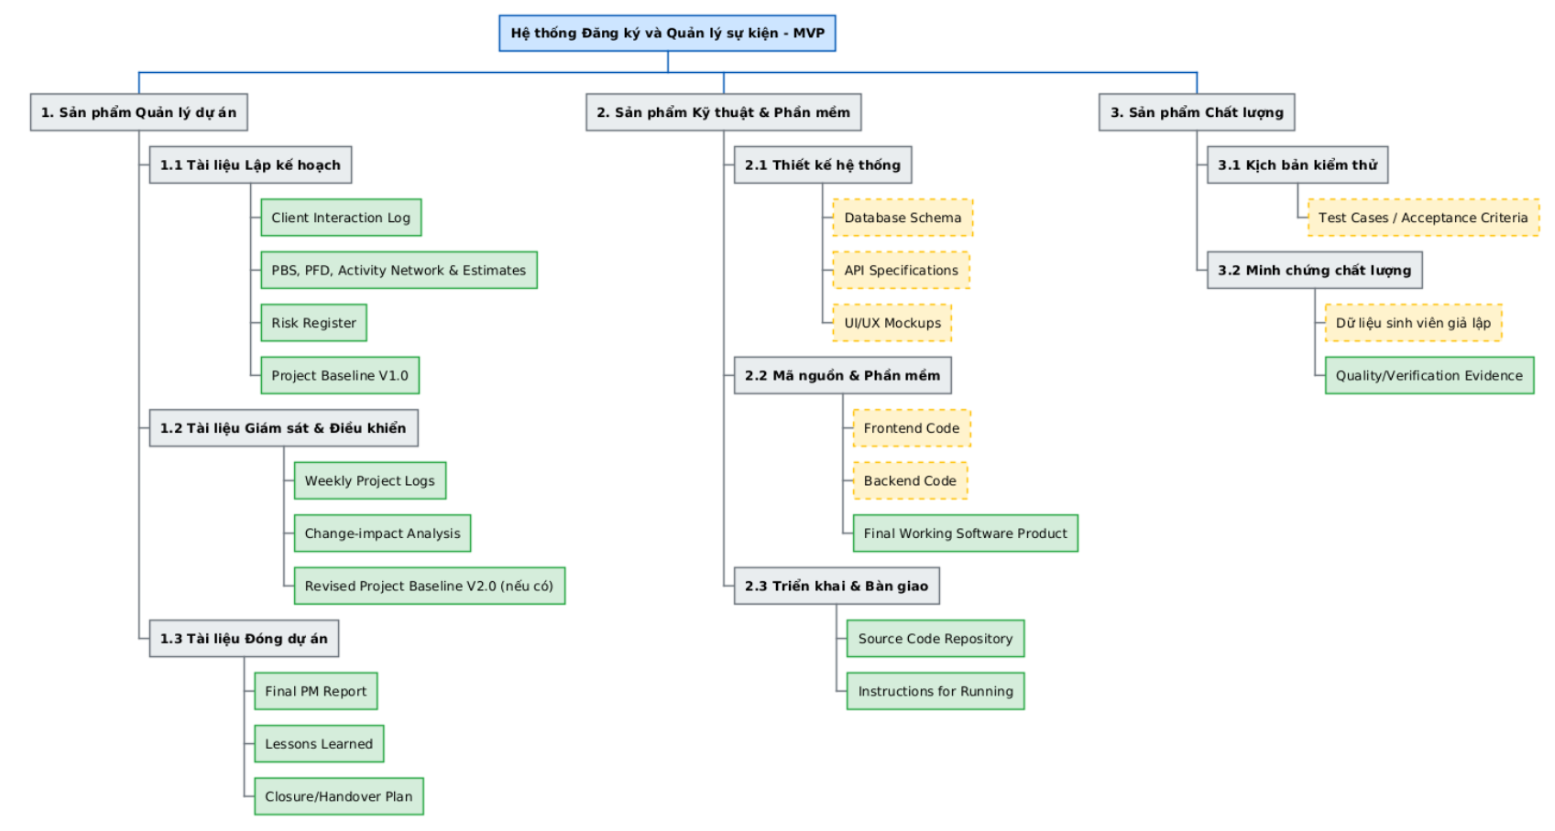
\includegraphics[width=\linewidth]{Images/PBS.png}
\end{adjustbox}
\captionsetup{aboveskip=3pt}
\caption{Cấu trúc phân rã sản phẩm của dự án}
\end{figure}

\noindent Ô xanh, viền liền: deliverable. Ô vàng, viền đứt: intermediate. Đường nối biểu diễn quan hệ phân rã, không biểu diễn thứ tự thực hiện.
\end{landscape}
\restoregeometry
\subsubsection{Phân biệt Deliverable products và Intermediate products}
Theo phương pháp Step Wise, việc phân định rõ hai loại sản phẩm này giúp nhóm tập trung nguồn lực vào các hạng mục cốt lõi cần nghiệm thu, đồng thời kiểm soát hiệu quả các công cụ hỗ trợ trong quá trình phát triển. Trong sơ đồ PBS, sự khác biệt này được trực quan hóa bằng màu sắc (xanh lá/vàng) và định dạng viền (liền/đứt). Căn cứ phân loại chi tiết được trình bày trong bảng sau:

\begin{table}[H]
\centering
\caption{Phân biệt sản phẩm bàn giao và sản phẩm trung gian}
\small
\renewcommand{\arraystretch}{1.25}
\begin{tabularx}{\textwidth}{|p{2cm}|>{\raggedright\arraybackslash}X|>{\raggedright\arraybackslash}X|}
\hline
\textbf{Tiêu chí} & \textbf{Sản phẩm bàn giao (Deliverable Products)(Ký hiệu: Ô màu xanh lá, nét liền)} & \textbf{Sản phẩm trung gian (Intermediate Products)(Ký hiệu: Ô màu vàng, nét đứt)} \\ \hline
Định nghĩa \& Tính chất & Là những sản phẩm đích bắt buộc phải hoàn thành và bàn giao để nghiệm thu ở các mốc của dự án. & Là các sản phẩm nội bộ, đóng vai trò làm đầu vào, công cụ kiểm soát hoặc thành phần cấu tạo để tạo ra sản phẩm bàn giao. \\ \hline
Căn cứ xác định & Xác định dựa trên danh sách "Expected outputs" và "Submission Requirements" của đề bài. Đây là minh chứng bắt buộc để đánh giá năng lực áp dụng quy trình quản lý dự án. & Xác định dựa trên quy trình phối hợp làm việc thực tế của nhóm (BA, Dev, QA) để xây dựng hệ thống. \\ \hline
Ví dụ nhóm Quản lý dự án & Toàn bộ tài liệu PM được xem là Deliverable vì là tiêu chí chấm điểm cốt lõi: Project Baseline V1.0, PBS, PFD, Estimates, Risk Register, Weekly Logs. & Các bản nháp, biên bản họp nội bộ (không yêu cầu nộp) được dùng để xây dựng kế hoạch chính thức. \\ \hline
Ví dụ nhóm Kỹ thuật \& Chất lượng & Final Working Software Product, Quality Evidence, Source Code Repository, Instructions for Running. & Database Schema, Mã nguồn Frontend/Backend, Test Cases, Dữ liệu giả lập. \\ \hline
\end{tabularx}
\end{table}
